\externaldocument{tech_eclipse_text}

\section{Visibility Calculations of Regions \label{vis}}
Recall that in order to calculate \fmod, the visibility of each region at a given time step is required. These visibilities are calculated by finding the projected surface area of a sphere for a given set of angles. The basic integral is the spherical surface integral dotted with the unit vector, $\hat{x}$, along the line-of-sight:

\begin{equation}
	V_{i,j} = \int_{\phi_1}^{\phi_2} \int_{\theta_1}^{\theta_2} \sin^2{\theta}\cos{\phi}\,\mathrm{d}\theta \, \mathrm{d}\phi
\end{equation}

\begin{figure}[h]
	\centering
	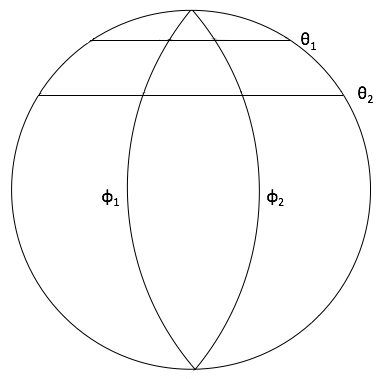
\includegraphics[width=.5\textwidth]{images/angles.png}
	\caption{Angles.}
	\label{angles}
\end{figure}

Where $\phi_1$, $\phi_2$, $\theta_1$, and $\theta_2$ are shown in Figure~\ref{angles}. For all types of visibilities, $\phi_1$ and $\phi_2$ are set by the number of stripes or boxes defined at the start of the program. The $\theta$ limits, however, will be different depending on region type.
The $\theta$ limits for the boxes are set by the impact parameter and the radius of the planet. The limits will be equal to $(b \pm R_p) + \frac{\pi}{2}$. The addition of $\frac{\pi}{2}$ is necessary when the bottom of the star is defined as latitude 0. For the visibility of a longitude, $\theta$ will range from 0 to $\pi$. The visibility of a stripe is calculated (in the chi-squared routine) by subtracting the sum of the box visibilities in a given longitude range from the longitude in the same range.